\documentclass[10pt,a4paper]{article}
\usepackage[utf8]{inputenc}
\usepackage{amsmath}
\usepackage{gensymb}
\usepackage{amsfonts}
\usepackage{siunitx}
\usepackage[european]{circuitikz}
\usepackage{geometry}
\newgeometry{tmargin=2cm, bmargin=2cm, lmargin=2cm, rmargin=2cm}
\usepackage{amssymb}
\usepackage{multirow}
\usepackage{polski}
\usepackage{graphicx}
\author{\textbf{T. Fąs}}
\title{\textbf{WZMACNIACZ OPERACYJNY}}
\begin{document}
\maketitle

\begin{center}
\textbf{\subsection*{STRESZCZENIE}}
\end{center}
W doświadczeniu zbadano właściwości wzmacniacza operacyjnego oraz skonstruowano układy oparte o ten wzmacniacz. Wszystkie konstrukcje zachowywały się zgodnie z oczekiwaniami.


\begin{center}
\textbf{\subsection*{WSTĘP}}
\end{center}
Wzmacniacz operacyjny jest układem realizującym operację wzmocnienia różnicy sygnałów wejściowych. Symbol wzmacniacza przedstawiony jest na Rysunku 1.

\begin{figure}[h!]
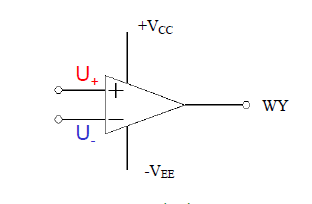
\includegraphics[width=6cm]{rap23rys1} 
\centering
\caption{Wzmacniacz operacyjny.}
\end{figure}

Jeżeli na wejście "+" znajduje się napięcie $U_{+}$, a na wejściu "-" napięcie $U_{-}$, to na wyjściu wzmacniacza otrzymamy sygnał $A(U_{+}-U_{-})$, gdzie $A$ jest pewną stałą wzmocnienia. Układ ten wymaga dodatkowo zasilania z dwóch źródeł, tu oznaczonych jako $V_{CC}$ i $V_{EE}$.


Korzystając z tego elementu można stworzyć: wzmacniacz odwracający fazę (sygnał na wyjściu ma przeciwną fazę), wzmacniacz nieodwracający fazy, układ różniczkujący (sygnał na wyjściu jest pochodną sygnału wejściowego) i układ całkujący. Schematy tych układów przedstawiono na Rysunku 2. 

\begin{figure}[h!]
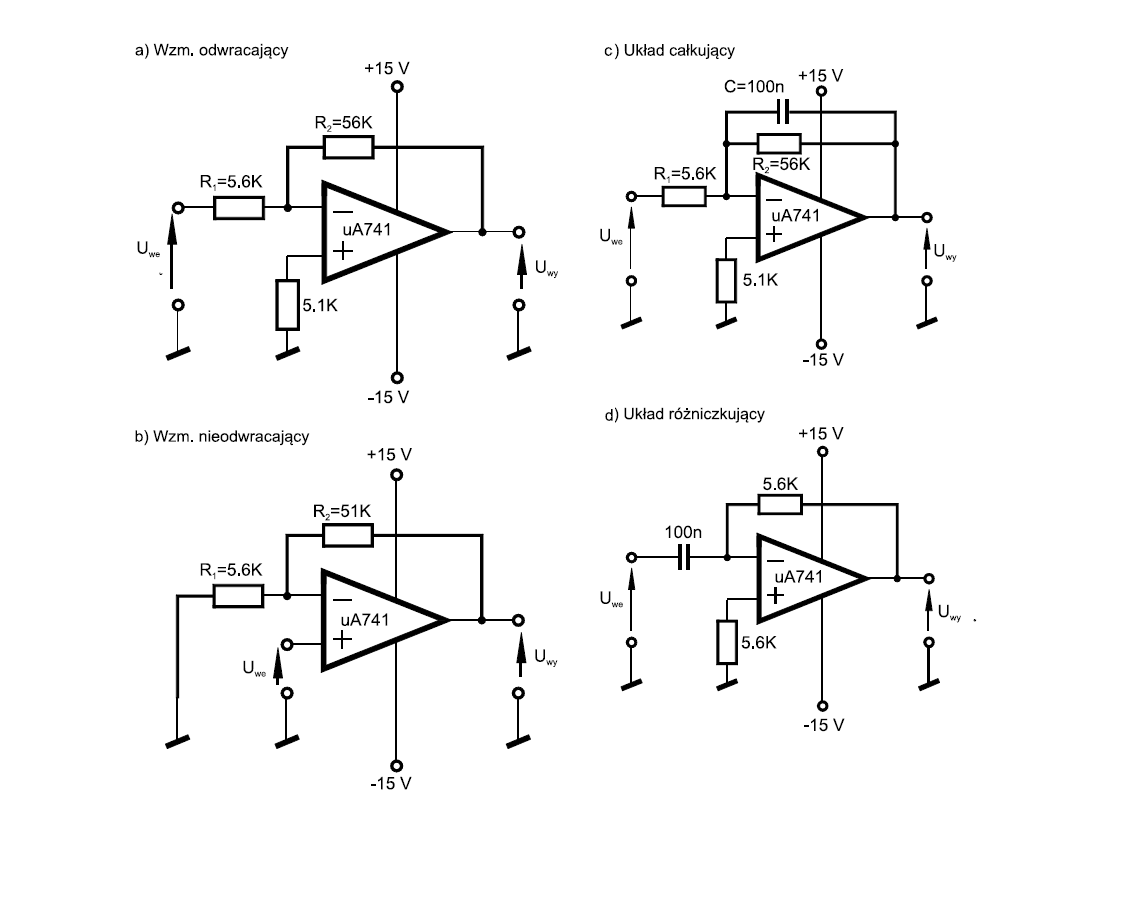
\includegraphics[width=12cm]{rap23rys2} 
\centering
\caption{Schematy układów \cite{r1}.}
\end{figure}

W przypadku wzmacniaczy, zależność napięcia wejściowego od wyjściowego jest zależnością liniową, a zależność napięcia wyjściowego $U_{wy}$ od częstości $\omega$ napięcia  wejściowego $U_{we}$ jest zależnością filtra dolnoprzepustowego, tj:

\begin{equation}
k=\left| \dfrac{U_{wy}}{U_{we}}\right|=\dfrac{k_{0}\omega_{g}}{\sqrt{\omega^2+\omega_{g}^2}},
\end{equation}

gdzie $k$ to stała wzmocnienia, a $\omega_{g}$ to częstość krytyczna, dla której stosunek napięć wynosi $1/\sqrt{2}$. 

\begin{center}
\textbf{\subsection*{UKŁAD DOŚWIADCZALNY}}
\end{center}
Układ doświadczalny składał się z: wzmacniacza operacyjnego uA741, oscyloskopu, zasilacza i oporników o rezystancji: 56,39, 5,55, 4,99, 52,35 i 5,08 k$\Omega$. Na Rysunku 2 znajdują się ich położenia w układzie i przybliżone wartości. Do wejścia +15 V podłączono wyjście + jednego z zasilaczy, a do wejścia -15 V podłączono wyjście - drugiego z zasilaczy. Wolne wyjścia kolejno - i + zasilaczy podłączono do wspólnego uziemienia. 



\begin{center}
\textbf{\subsection*{WYNIKI POMIARÓW}}
\end{center}

 Dokonano pomiarów zależności wzmocnienia $k$ od amplitudy napięcia wejściowego przy stałej częstości 1 kHz oraz zależności wzmocnienia od częstości przy stałej amplitudzie 1 V sygnału wejściowego. Wyniki te dla wzmacniacza odwracającego i nieodwracającego przedstawiono kolejno w Tabeli 1 i Tabeli 2.
 
 W przypadku wzmacniacza odwracającego sygnał wyjściowy był przesunięty w fazie o $\pi$, co zmieniało znak sygnału na przeciwny, jednak w analizie danych przyjęto wartość bezwzględną  amplitudy. 
 
\begin{table}[h!]
\centering
\caption{Wyniki pomiarów: wzmocnienie od amplitudy.}
\begin{tabular}{|c|c|c|c|}
\hline
\multicolumn{2}{|c|}{Wzmacniacz odwracający} & \multicolumn{2}{c|}{Wzmacniacz nieodwracający} \\ \hline
$U_{we}$ [V]          & $U_{wy}$ [V]         & $U_{we}$ [V]           & $U_{wy}$ [V]          \\ \hline
0.01                  & 0.045                & 0.01                   & 0.11                  \\ \hline
0.0124                & 0.105                & 0.023                  & 0.216                 \\ \hline
0.0214                & 0.208                & 0.054                  & 0.528                 \\ \hline
0.0418                & 0.412                & 0.084                  & 0.84                  \\ \hline
0.0616                & 0.612                & 0.105                  & 1.06                  \\ \hline
0.0816                & 0.809                & 0.206                  & 2.12                  \\ \hline
1.02                  & 10.2                 & 0.508                  & 5.28                  \\ \hline
1.22                  & 12.3                 & 0.824                  & 8.48                  \\ \hline
1.42                  & 14.2                 & 1.02                   & 10.6                  \\ \hline
1.61                  & 16.3                 & 1.22                   & 12.6                  \\ \hline
1.82                  & 18.2                 & 1.42                   & 14.9                  \\ \hline
2.02                  & 20.4                 & 1.64                   & 16.8                  \\ \hline
2.2                   & 22.2                 & 1.88                   & 19.2                  \\ \hline
2.42                  & 24.4                 & 2.04                   & 21                    \\ \hline
2.62                  & 26.1                 & 2.24                   & 23                    \\ \hline
2.82                  & 26.9                 & 2.44                   & 25.4                  \\ \hline
3.02                  & 27.3                 & 2.66                   & 26.6                  \\ \hline
3.22                  & 27.3                 & 2.84                   & 27.2                  \\ \hline
3.42                  & 27.3                 & 3.06                   & 27.2                  \\ \hline
3.72                  & 27.3                 & 3.24                   & 27.2                  \\ \hline
4.04                  & 27.3                 & 3.46                   & 27.2                  \\ \hline
                      &                      & 3.66                   & 27.2                  \\ \hline
                      &                      & 3.86                   & 27.2                  \\ \hline
                      &                      & 4.06                   & 27.2                  \\ \hline
\end{tabular}
\end{table}



\begin{table}[h!]
\centering
\caption{Wyniki pomiarów: wzmocnienie od częstości.}
\begin{tabular}{|c|c|c|c|c|c|}
\hline
\multicolumn{3}{|c|}{Wzmacniacz odwracający} & \multicolumn{3}{c|}{Wzmacniacz nieodwracający} \\ \hline
$f$ [Hz]   & $U_{we}$ [V]   & $U_{wy}$ [V]   & $f$ [Hz]    & $U_{we}$ [V]    & $U_{wy}$ [V]   \\ \hline
10         & 1.04           & 10.6           & 10          & 1.06            & 10.8           \\ \hline
20         & 1.06           & 10.6           & 20          & 1.06            & 10.8           \\ \hline
50         & 1.06           & 10.6           & 50          & 1.06            & 10.8           \\ \hline
80         & 1.06           & 10.6           & 80          & 1.06            & 10.8           \\ \hline
100        & 1.03           & 10.2           & 100         & 1.06            & 10.8           \\ \hline
200        & 1.02           & 10.2           & 200         & 1.06            & 10.8           \\ \hline
500        & 1.02           & 10.2           & 500         & 1.06            & 10.8           \\ \hline
800        & 1.02           & 10.2           & 800         & 1.06            & 10.8           \\ \hline
1000       & 1.02           & 10.2           & 1000        & 1.06            & 10.8           \\ \hline
2000       & 1.02           & 10.2           & 2000        & 1.03            & 10.5           \\ \hline
5000       & 1.01           & 10.2           & 5000        & 1.02            & 10.5           \\ \hline
8000       & 1.01           & 10.2           & 8000        & 1.02            & 10.5           \\ \hline
10000      & 1.01           & 10.2           & 10000       & 1.02            & 10.5           \\ \hline
20000      & 1.01           & 9.92           & 20000       & 1.02            & 10.3           \\ \hline
50000      & 1.02           & 6.64           & 50000       & 1.02            & 6.64           \\ \hline
80000      & 1.02           & 4.24           & 80000       & 1.02            & 4.28           \\ \hline
100000     & 1.02           & 3.39           & 100000      & 1.02            & 3.44           \\ \hline
200000     & 1.01           & 1.71           & 200000      & 1.02            & 1.72           \\ \hline
500000     & 1.02           & 0.7            & 500000      & 1.02            & 0.7            \\ \hline
800000     & 1.02           & 0.44           & 800000      & 1.02            & 0.437          \\ \hline
1000000    & 1.02           & 0.34           & 1000000     & 1.02            & 0.351          \\ \hline
1200000    & 1.02           & 0.28           & 1300000     & 1.01            & 0.266          \\ \hline
1400000    & 1.02           & 0.244          & 1600000     & 1.01            & 0.206          \\ \hline
1600000    & 1.02           & 0.206          & 1900000     & 1.01            & 0.182          \\ \hline
1800000    & 1.01           & 0.18           & 2000000     & 1.01            & 0.168          \\ \hline
2000000    & 1.01           & 0.168          &             &                 &                \\ \hline
\end{tabular}
\end{table}

Zbadano również zachowanie układu różniczkującego i całkującego. Zgodnie z oczekiwaniami zamieniały one kolejno sygnał trójkątny na prostokątny i sygnał prostokątny na trójkątny. 
Zmierzono też przedziały dobrego całkowania/różniczkowania dla tych układów. Otrzymano przedział 150 Hz - 150 kHz dla układu całkującego i 40 Hz - 1 kHz dla różniczkującego.

\begin{center}
\textbf{\subsection*{ANALIZA DANYCH}}
\end{center}

Na podstawie danych z Tabeli 1 wykonano wykres zależności współczynnika wzmocnienia $k$ od amplitudy sygnału wejściowego. Wykresy te przedstawiono na Rysunku 3 i Rysunku 4.

\begin{figure}[h!]
\centering
\begin{minipage}{0.5\textwidth}
  \centering
  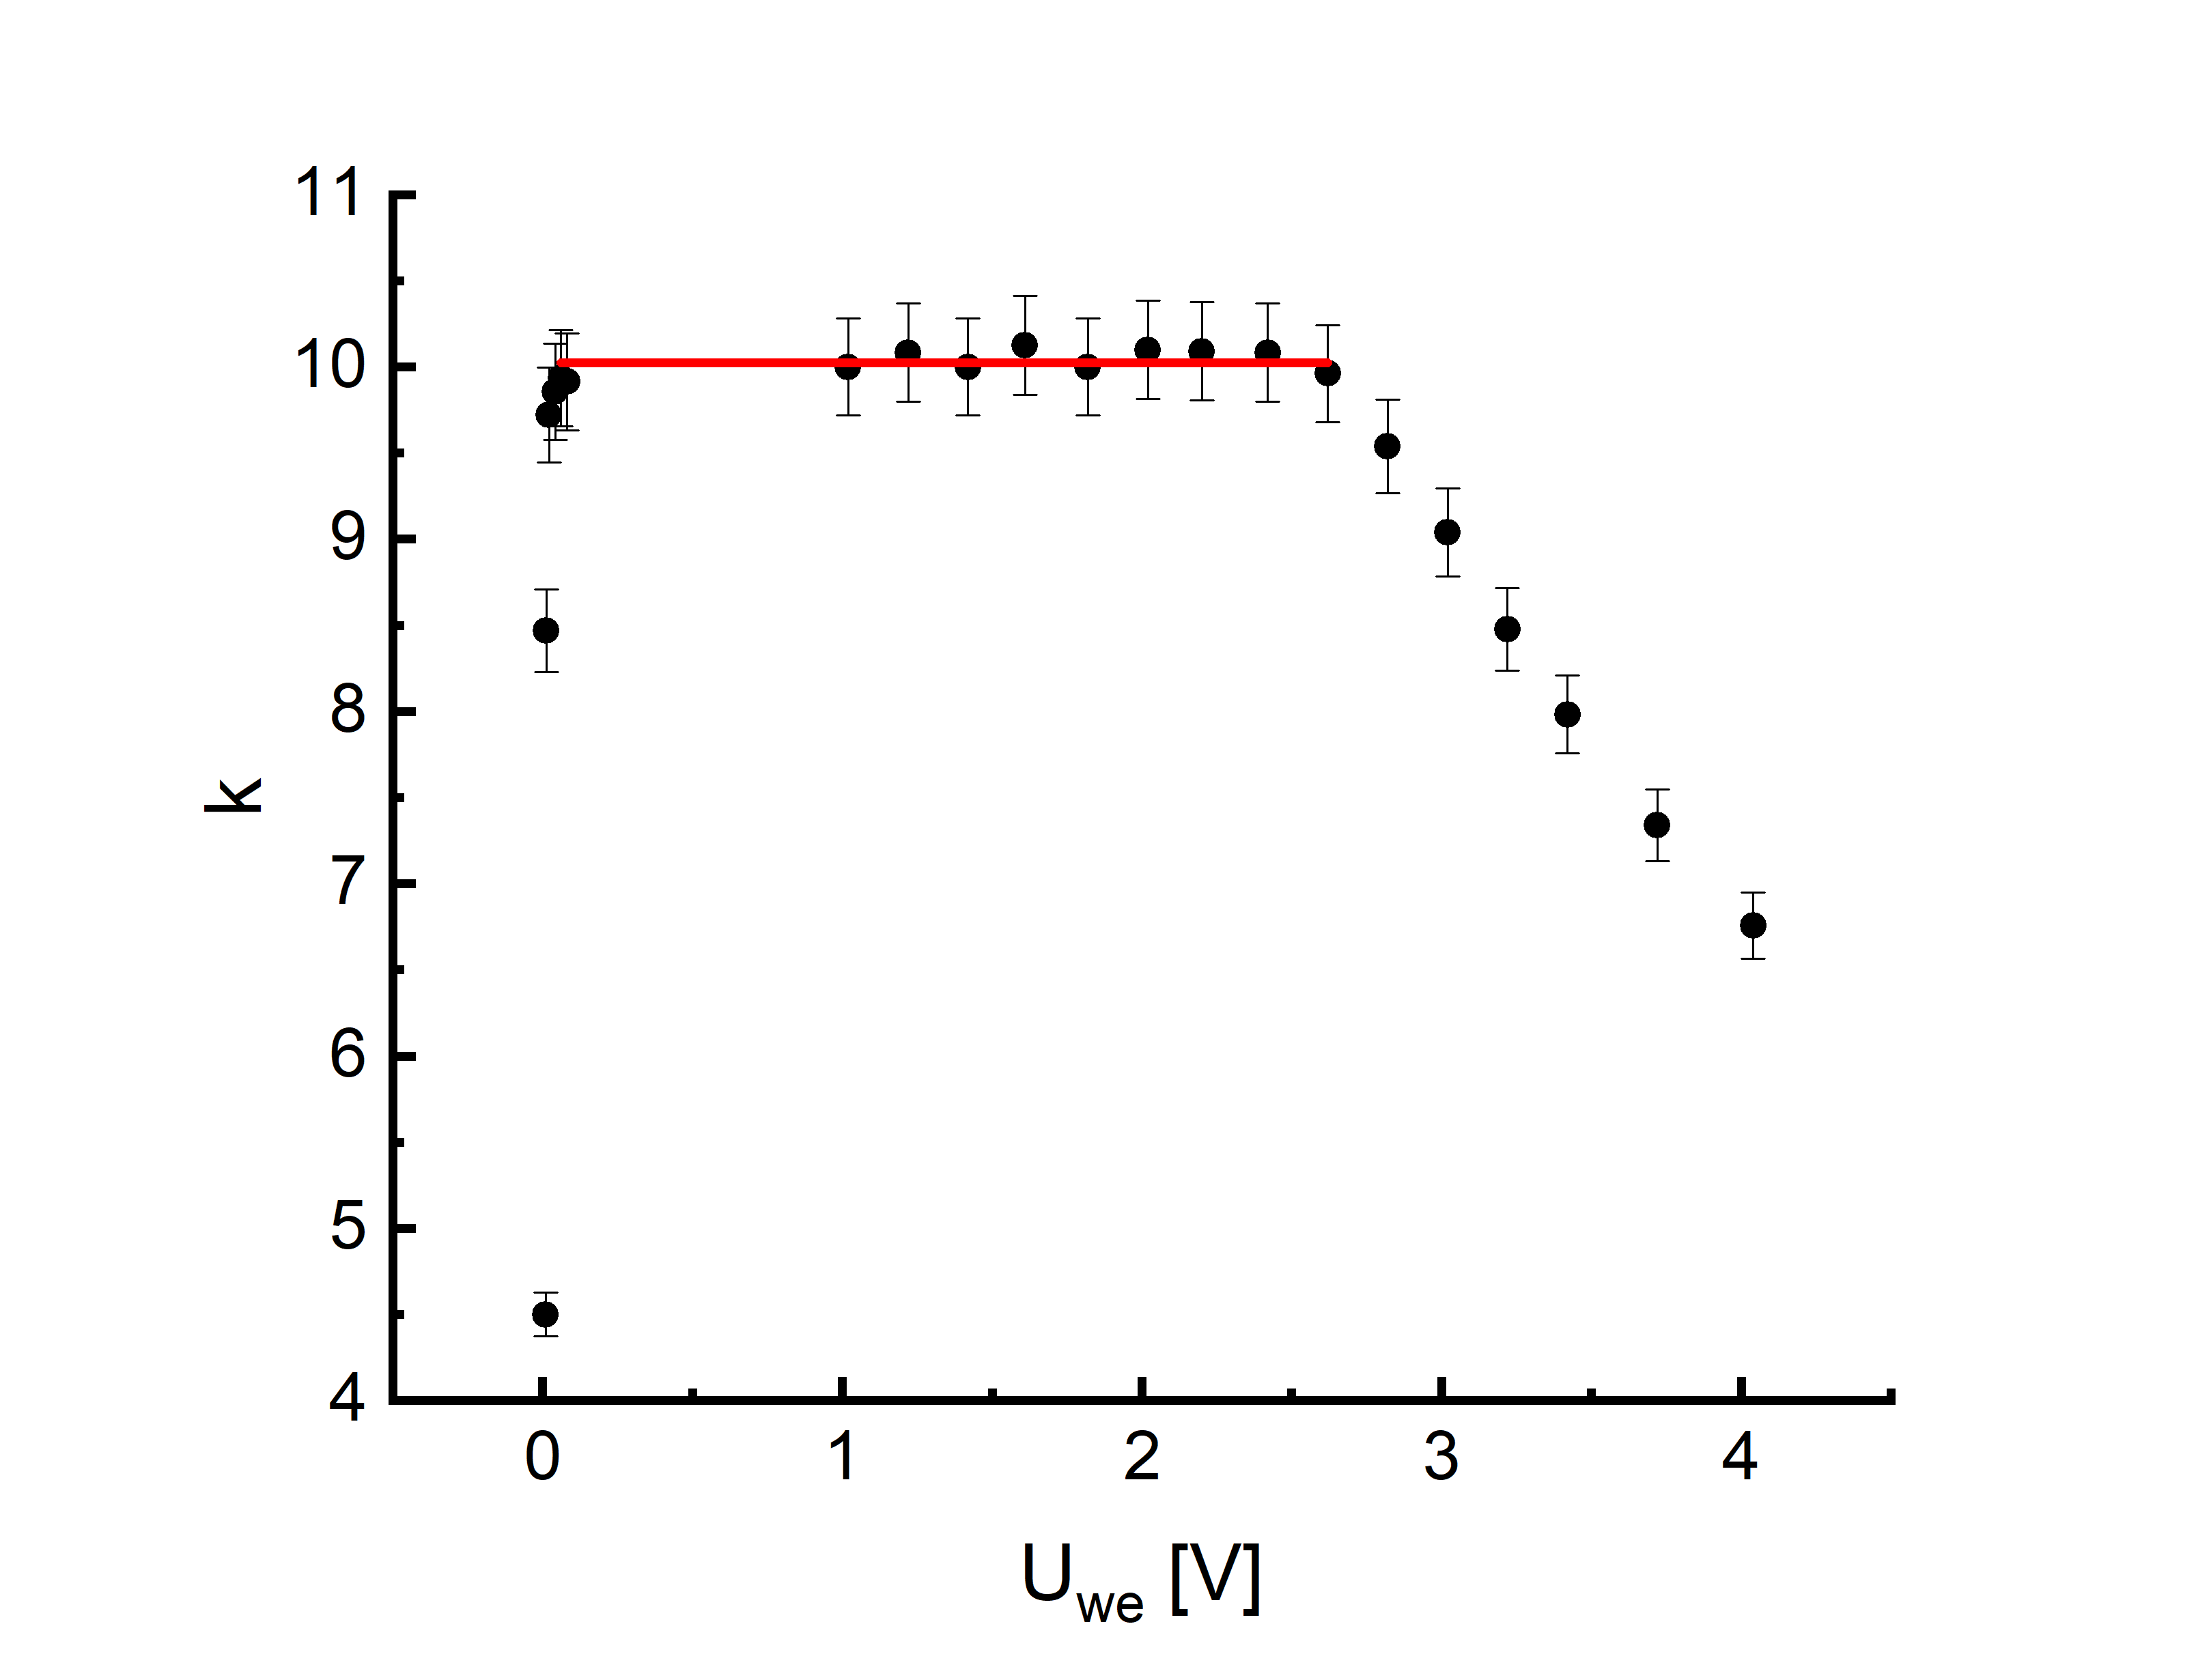
\includegraphics[width=10cm, height=8cm ]{rap23rys3} 
\caption{$k(U_{we})$: wzmacniacz odwracający.}
\end{minipage}%
\begin{minipage}{0.5\textwidth}
  \centering
  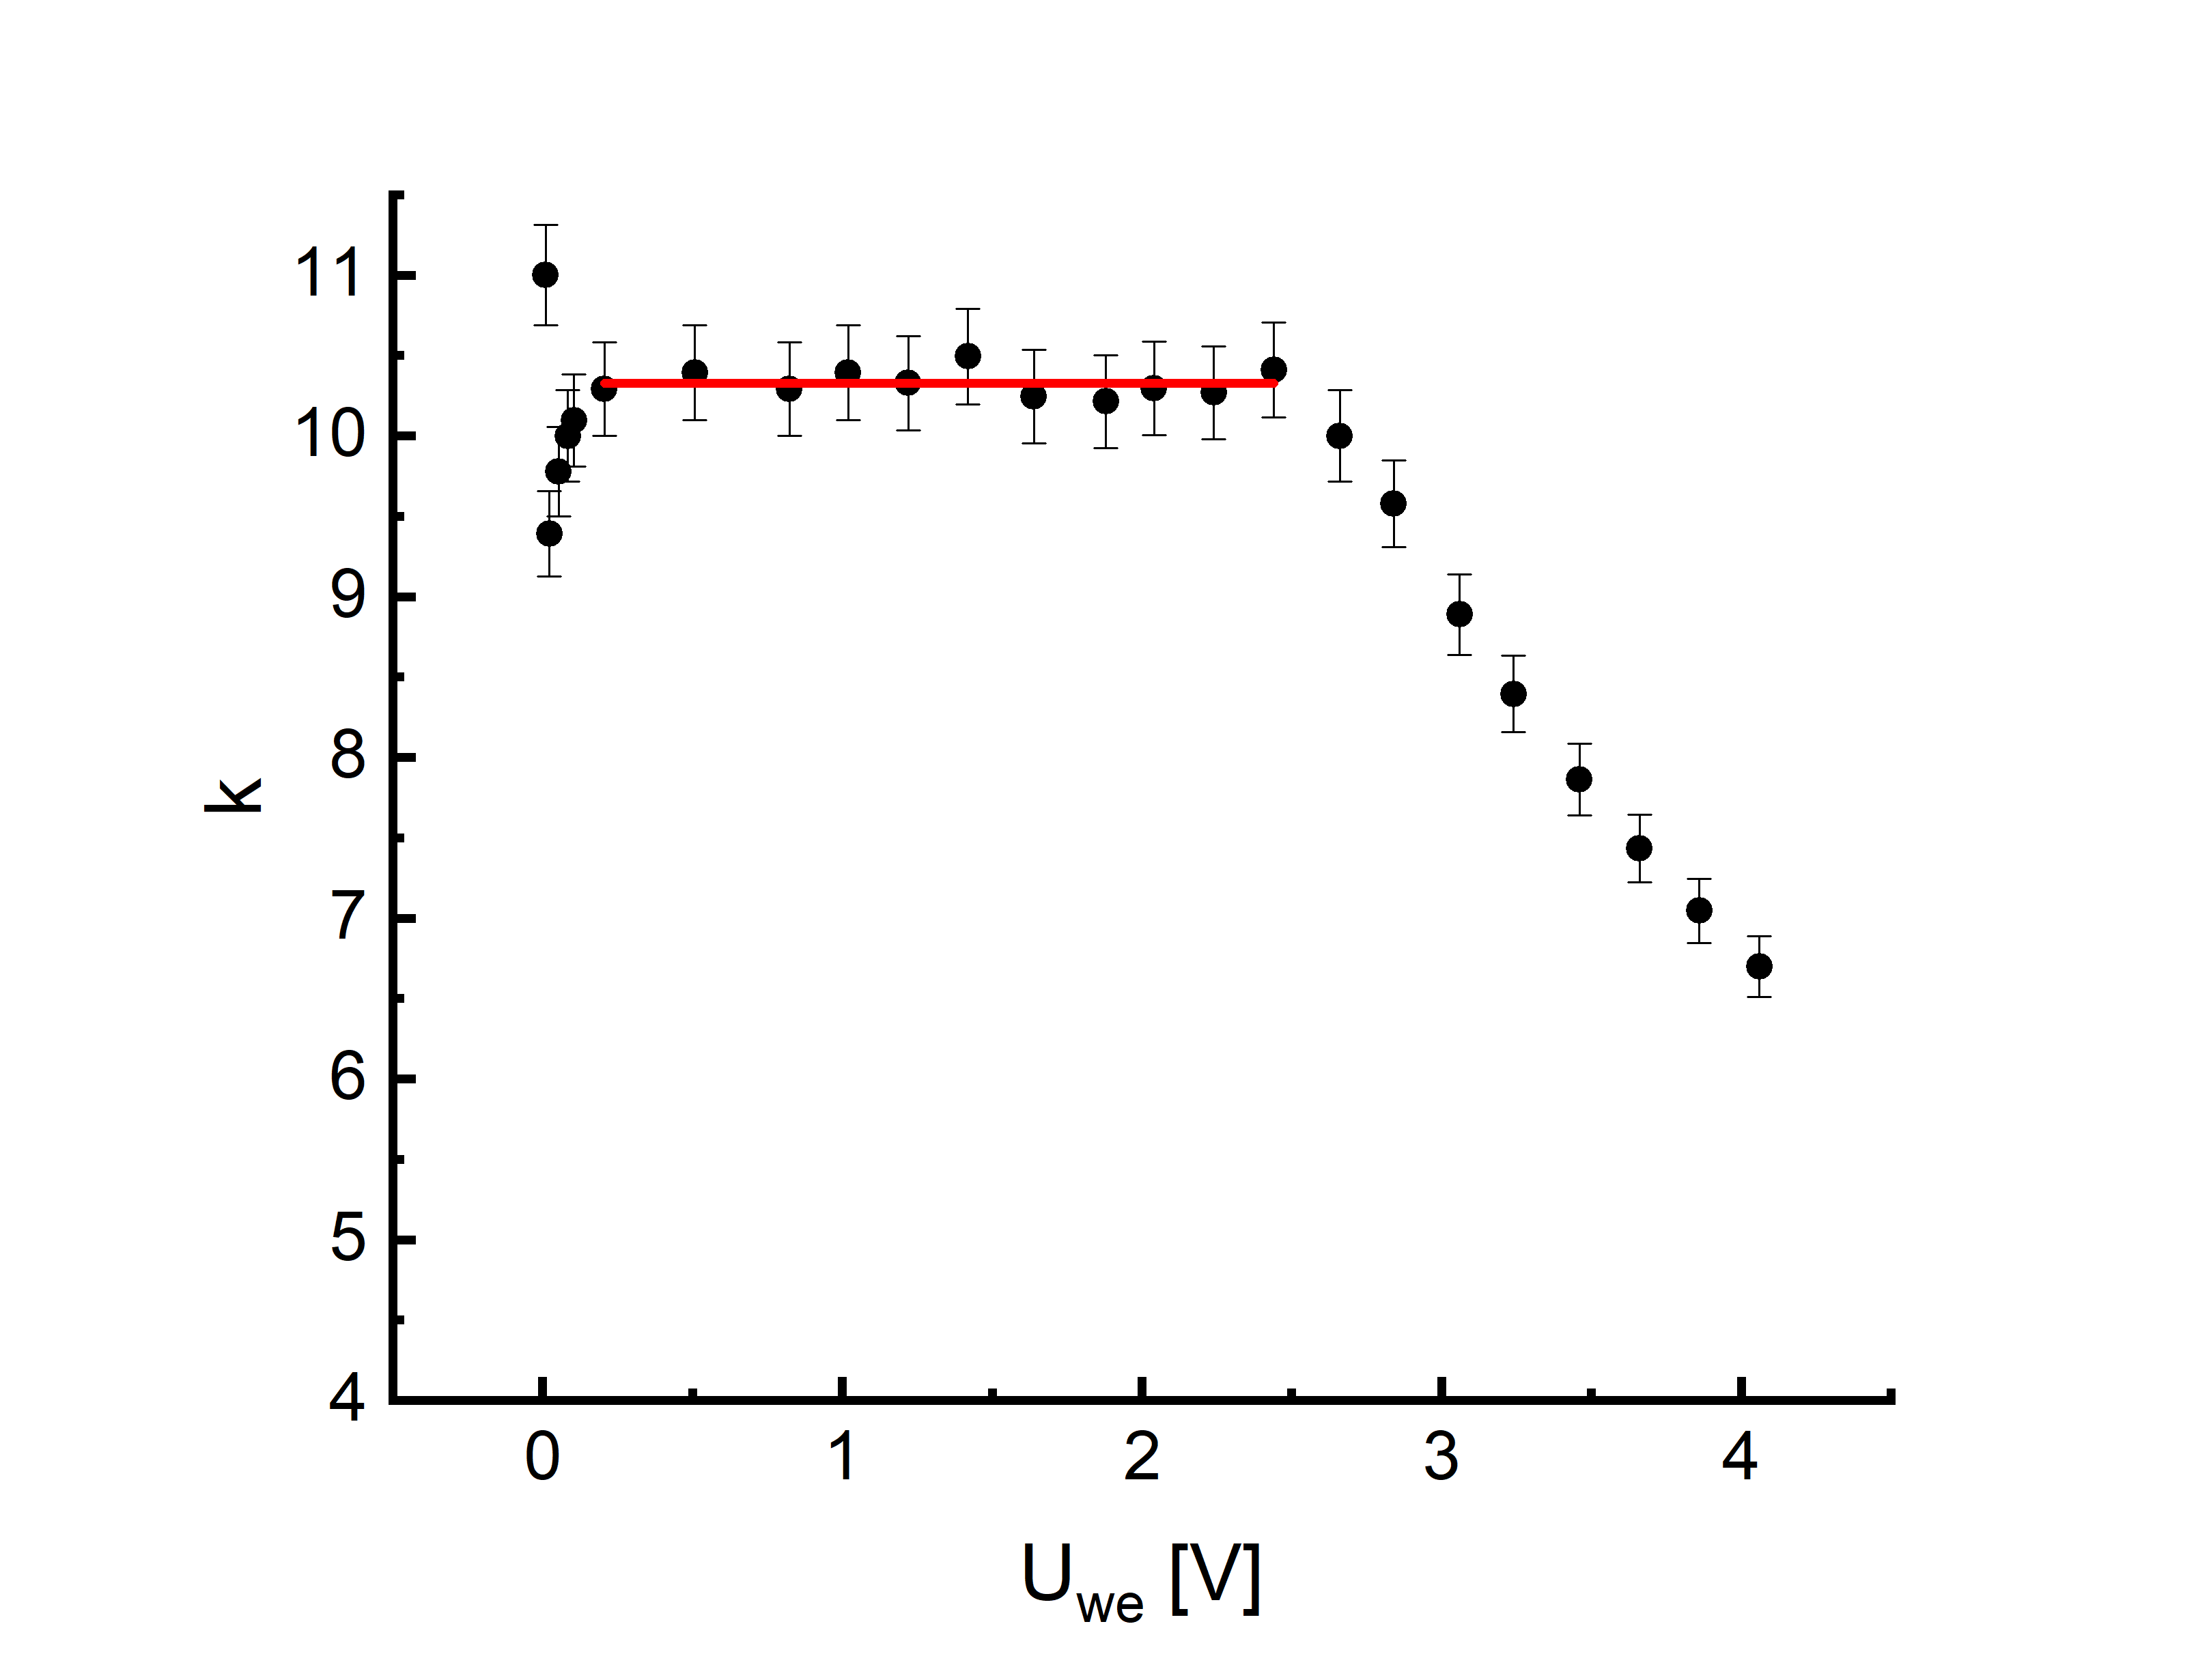
\includegraphics[width=10cm, height=8cm ]{rap23rys4} 
\caption{$k(U_{we})$: wzmacniacz nieodwracający.}
\end{minipage}
\end{figure}

Do danych dopasowano funkcję stałą w przedziale stałego wzmocnienia. Przyjęto wartości błędów równe 2\% dla pomiarów napięcia. Otrzymano wartości $k_{0}=10,025\pm0,022$ dla wzmacniacza odwracającego i przedziału (0,0616:2,62) V oraz $k_{0}=10,328\pm0,025$ dla nieodwracającego w przedziale (0,206:2,44) V.

Teoretyczne wartości bezwzględne wzmocnienia dla wzmacniacza odwracającego i nieodwracającego to kolejno $R_{2}/R_{1}$ i $1+R_{2}/R_{1}$, co po podstawieniu zmierzonych wartości oporu daje wzmocnienia $10,16\pm0,29$ i $10,43\pm0,30$. Założono błąd pomiaru oporu jako 2\%. Wartości te są zgodne z wartościami otrzymanymi eksperymentalnie, otrzymano rozbieżność wyników kolejno 0,38$\sigma$ i 0,28$\sigma$, gdzie $\sigma$ to to pierwiastek z sumy kwadratów niepewności.

Na podstawie danych z Tabeli 2 wykonano wykresy zależności wzmocnienia $k$ od częstości $\omega=2\pi f$. Wykresy przedstawiono na Rysunku 5 i Rysunku 6. 

\begin{figure}[h!]
\centering
\begin{minipage}{0.5\textwidth}
  \centering
  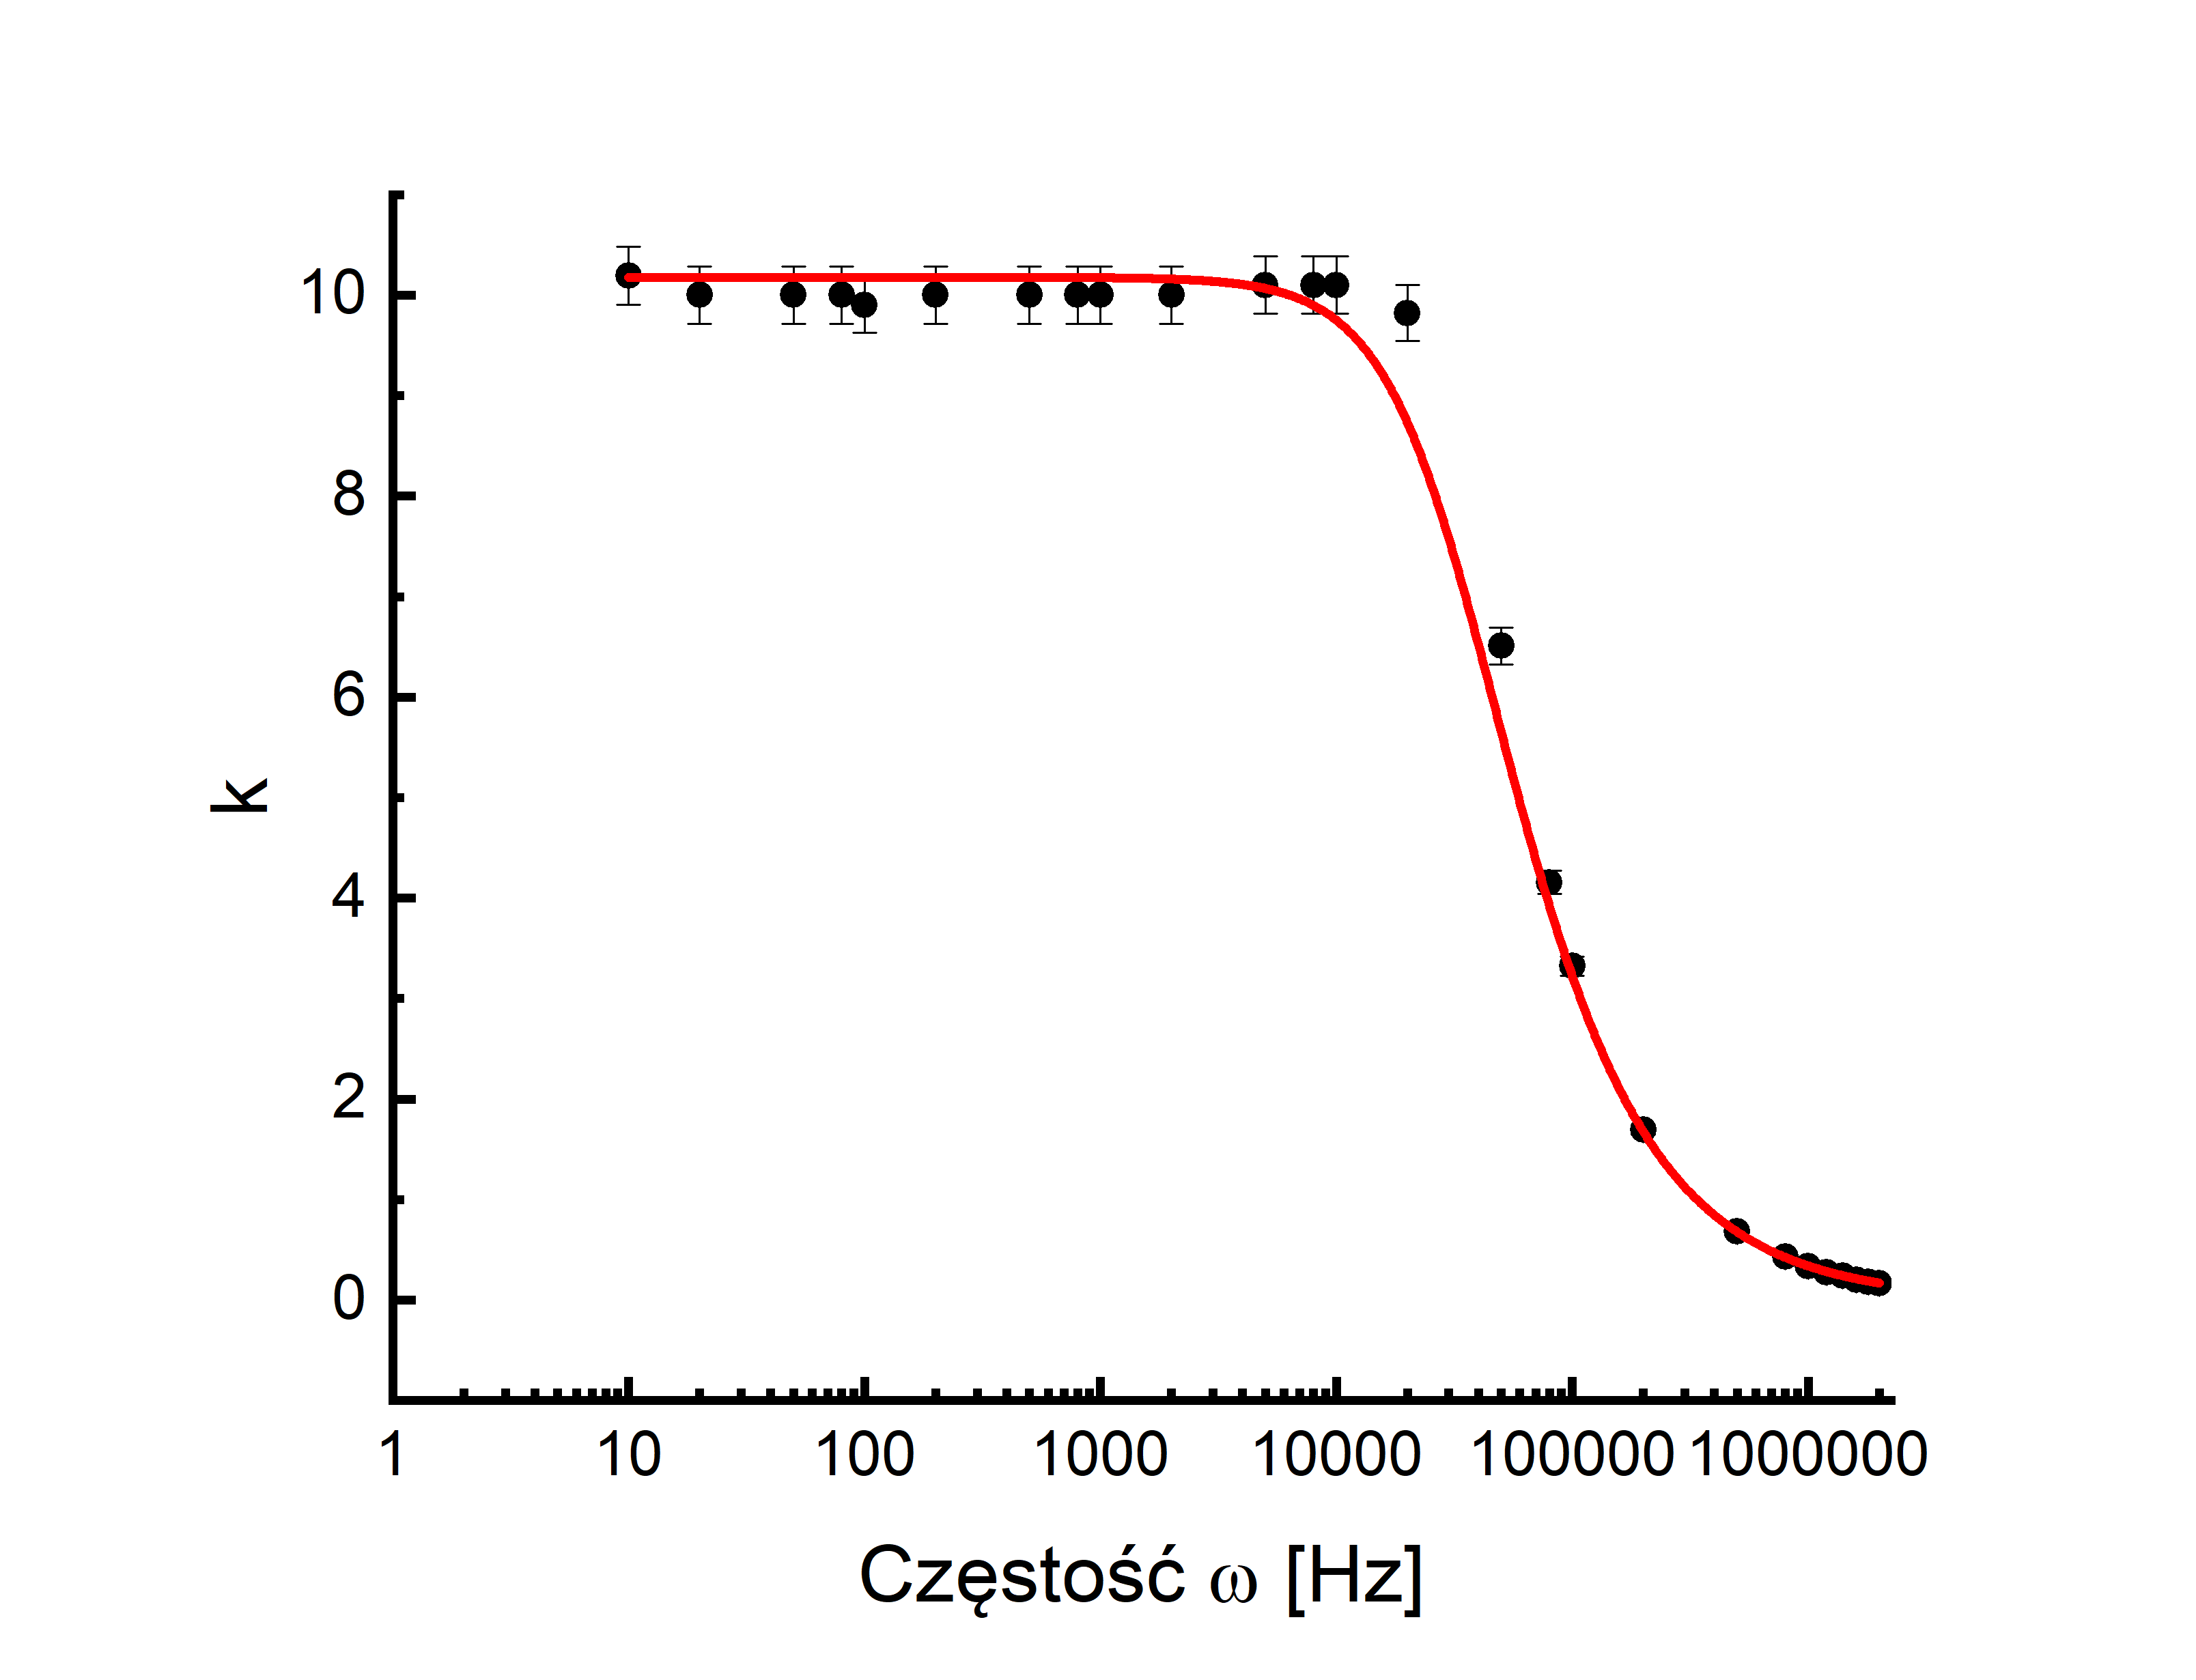
\includegraphics[width=9cm, height=8cm ]{rap23rys5} 
\caption{$k(\omega)$: wzmacniacz odwracający.}
\end{minipage}%
\begin{minipage}{0.5\textwidth}
  \centering
  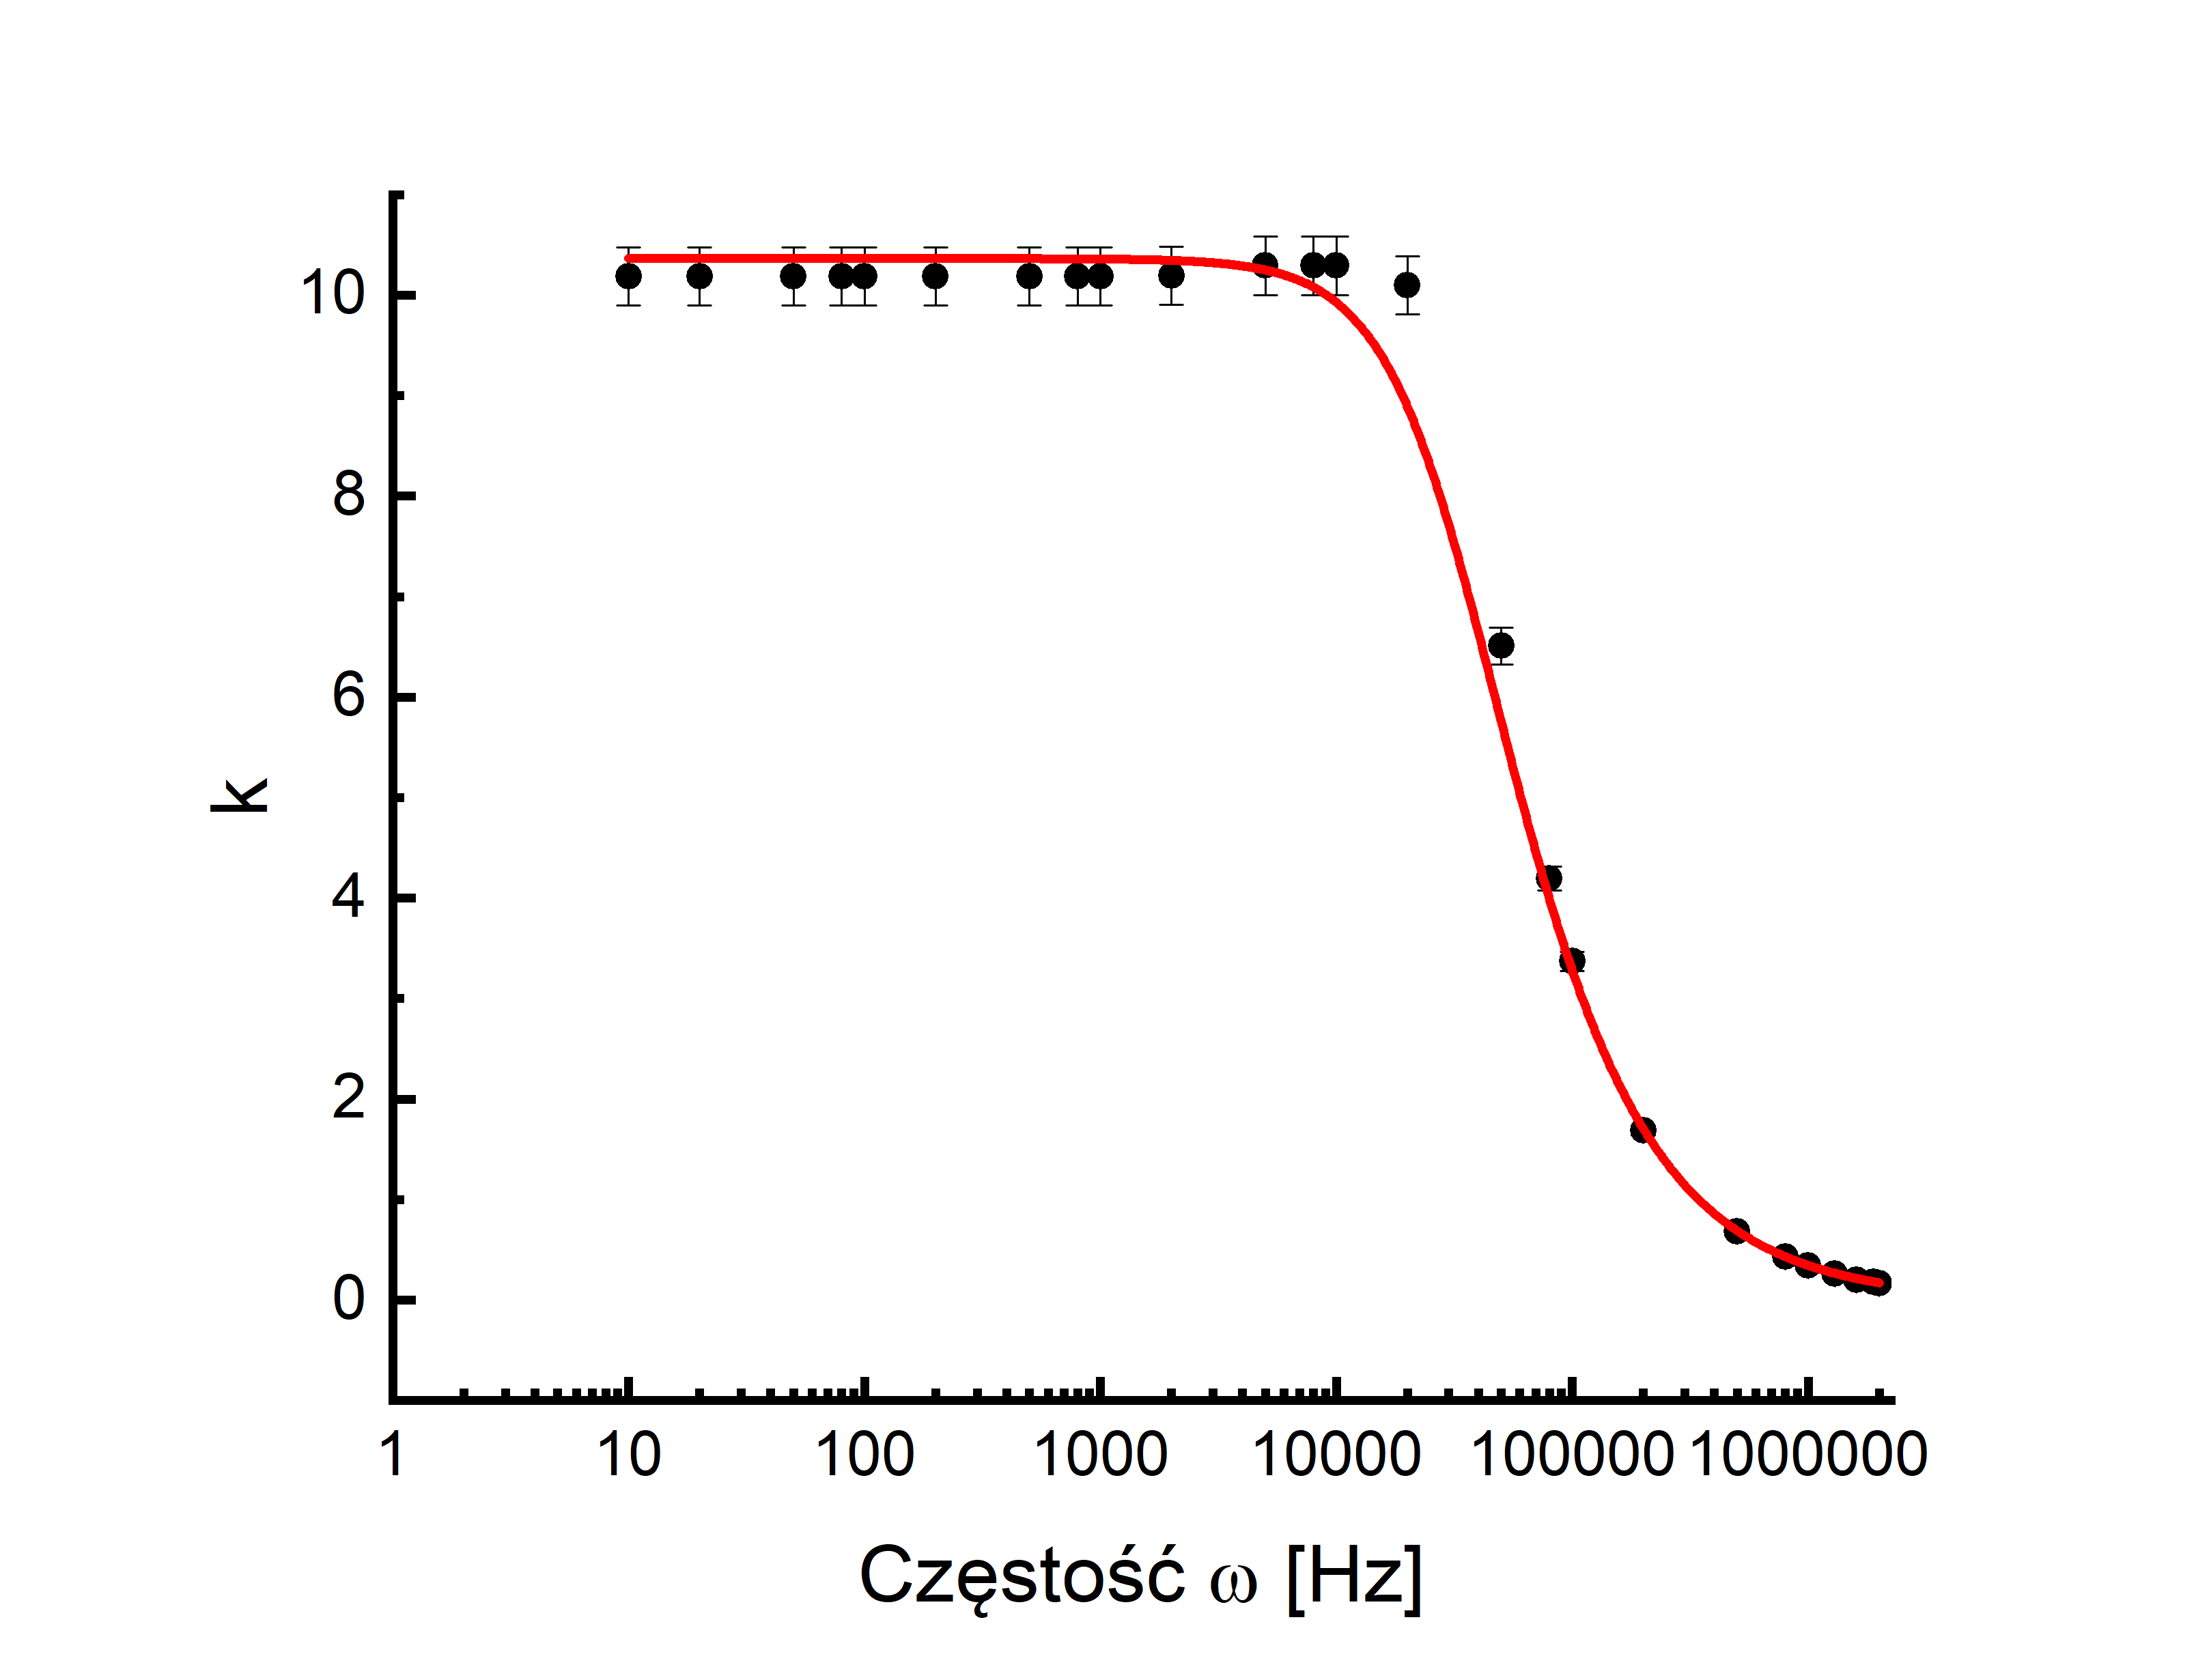
\includegraphics[width=9cm, height=8cm ]{rap23rys6} 
\caption{$k(\omega)$: wzmacniacz nieodwracający.}
\end{minipage}
\end{figure}

Do punktów pomiarowych dopasowano zależność z Równania (1), zakładając błąd pomiaru napięcia równy 2\%. Otrzymano wartości dopasowania: $k_{0}=10,18\pm0,12$ i $\omega_{g}=33400\pm620$ s$^{-1}$ dla wzmacniacza odwracającego oraz $k_{0}=10,36\pm0,12$ i $\omega_{g}=33400\pm600$ s$^{-1}$ dla nieodwracającego. Wartości $k_{0}$ są zgodne z wcześniej otrzymanymi wynikami.

\begin{center}
\textbf{\subsection*{DYSKUSJA WYNIKÓW I WNIOSKI}}
\end{center} 

Otrzymane wartości wzmocnień były ze sobą zgodne jak i byłe zgodne z wartościami teoretycznymi. To samo tyczy się otrzymanych charakterystyk jak i własności różniczkujących i całkujących. Podsumowując: doświadczenie przebiegło pomyślnie.


\begin{center}
\begin{thebibliography}{9}

\bibitem{r1}
 Praca zbiorowa,
 \emph{Instrukcja do ćwiczenia "Wzmacniacz operacyjny"},
 FUW, Warszawa, 2016.
 
 
 
 \end{thebibliography}

\end{center}


\end{document}